\section{Neural Network Architectures}
\begin{frame}{What We Choose When Building a Neural Network}
\textbf{Key Design Decisions:}
\vspace{0.5em}

\begin{columns}[t]
\begin{column}{0.48\textwidth}
\begin{tcolorbox}[colback=blue!5, colframe=blue!50, title=\textbf{1. Model Architecture}]
\textbf{Structure:}
\begin{itemize}
\item Number of layers
\item Neurons per layer
\item Network type (MLP/CNN/RNN)
\end{itemize}
\vspace{0.3em}
\textbf{Components:}
\begin{itemize}
\item Activation functions (ReLU, sigmoid, tanh)
\item Output layer shape \& activation
\end{itemize}
\end{tcolorbox}
\end{column}

\begin{column}{0.48\textwidth}
\begin{tcolorbox}[colback=green!5, colframe=green!50!black, title=\textbf{2. Training Strategy}]
\textbf{Learning:}
\begin{itemize}
\item Loss function (MSE, cross-entropy)
\item Optimizer (SGD, Adam, AdamW)
\end{itemize}
\vspace{0.3em}
\textbf{Hyperparameters:}
\begin{itemize}
\item Learning rate
\item Batch size
\item Number of epochs
\end{itemize}
\end{tcolorbox}
\end{column}
\end{columns}
\end{frame}


\section{Types of Neural Network Architectures}

% =========================
% 6. Architectures and Autoencoders
% =========================
\begin{frame}{Types of Neural Network Architectures}
    \begin{itemize}
        \item \textbf{MLP} fully connected network for tabular data
        \item \textbf{CNN} convolutional neural network for images
        \item \textbf{RNN and variants} for sequences and time series
    \end{itemize}
    \vspace{1em}
    \begin{figure}
        \centering
        % Replace with a clear figure that compares MLP, CNN, RNN
        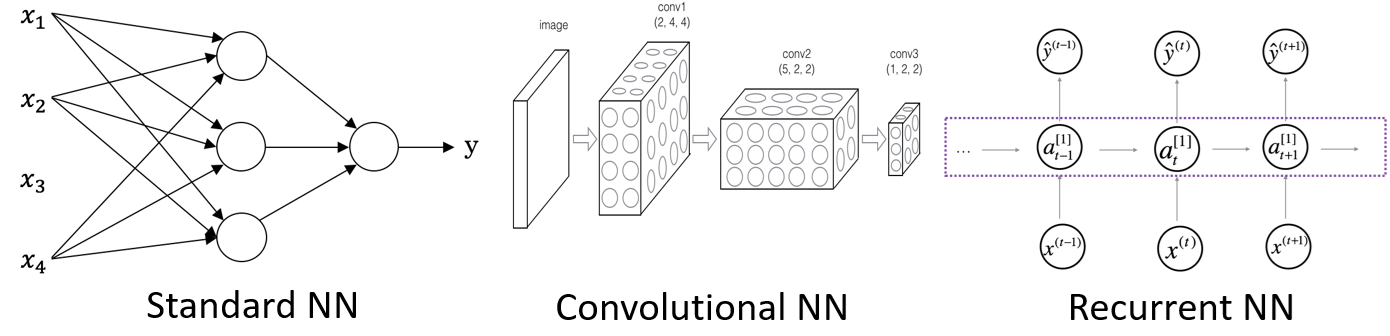
\includegraphics[width=\textwidth,height=0.6\textheight,keepaspectratio]{images/nn_types.png}
    \end{figure}
\end{frame}


% =========================
% References
% =========================

\section{References}
